%%%%%%%%%%%%%%%%%%%%%%%%%%%%%%%%%%%%%%%%%
% Original:
% Computational Physics and Biophysics Group, Jacobs University
% https://teamwork.jacobs-university.de:8443/confluence/display/CoPandBiG/LaTeX+Poster
% 
% This template has been downloaded from:
% http://www.LaTeXTemplates.com
%
% License:
% CC BY-NC-SA 3.0 (http://creativecommons.org/licenses/by-nc-sa/3.0/)
%
%%%%%%%%%%%%%%%%%%%%%%%%%%%%%%%%%%%%%%%%%

%----------------------------------------------------------------------------------------
%	PACKAGES AND OTHER DOCUMENT CONFIGURATIONS
%----------------------------------------------------------------------------------------

\documentclass[final]{beamer}

\usepackage[scale=1.5]{beamerposter} % Use the beamerposter package for laying out the poster
\usepackage{caption}
\usepackage{subcaption}
\usepackage{braket}
\usepackage{amsmath}
% \usepackage{ragged2e}
\usepackage{lipsum}
\usepackage{bm}


\usetheme{confposter} % Use the confposter theme supplied with this template

% \setbeamertemplate{block title}[]{}

\setbeamercolor{block title}{fg=ddblue,bg=white} % Colors of the block titles
\setbeamercolor{block body}{fg=black,bg=white} % Colors of the body of blocks
\setbeamercolor{block alerted title}{fg=white,bg=ddblue} % Colors of the highlighted block titles
\setbeamercolor{block alerted body}{fg=black,bg=black!10} % Colors of the body of highlighted blocks
% Many more colors are available for use in beamerthemeconfposter.sty

\setbeamertemplate{caption}[numbered]

\binoppenalty=10000
\relpenalty=10000


%-----------------------------------------------------------
% Define the column widths and overall poster size
% To set effective sepwid, onecolwid and twocolwid values, first choose how many columns you want and how much separation you want between columns
% In this template, the separation width chosen is 0.024 of the paper width and a 4-column layout
% onecolwid should therefore be (1-(# of columns+1)*sepwid)/# of columns e.g. (1-(4+1)*0.024)/4 = 0.22
% Set twocolwid to be (2*onecolwid)+sepwid = 0.464
% Set threecolwid to be (3*onecolwid)+2*sepwid = 0.708

\newlength{\sepwid}
\newlength{\onecolwid}
\newlength{\twocolwid}
\newlength{\threecolwid}
\setlength{\paperwidth}{48in} % A0 width: 46.8in
\setlength{\paperheight}{36in} % A0 height: 33.1in
\setlength{\sepwid}{0.024\paperwidth} % Separation width (white space) between columns
\setlength{\onecolwid}{0.22\paperwidth} % Width of one column
\setlength{\twocolwid}{0.464\paperwidth} % Width of two columns
\setlength{\threecolwid}{0.708\paperwidth} % Width of three columns
\setlength{\topmargin}{-0.5in} % Reduce the top margin size
%-----------------------------------------------------------

\usepackage{graphicx}  % Required for including images
\usepackage{booktabs} % Top and bottom rules for tables

%----------------------------------------------------------------------------------------
%	TITLE SECTION 
%----------------------------------------------------------------------------------------

\title{Quantum vs Classical Local Algorithms for Local MaxCut}

\author{\texorpdfstring{Adam Bouland$^\dagger$, Charlie Carlson$^*$, Alex Kolla$^*$, Steven Kordonowy$^*$}{Foo}}

\institute{University of Colorado - Boulder ($^*$), Stanford University ($^\dagger$)}
%----------------------------------------------------------------------------------------

\begin{document}
  
\addtobeamertemplate{block end}{}{\vspace*{2ex}} % White space under blocks
\addtobeamertemplate{block alerted end}{}{\vspace*{2ex}} % White space under highlighted (alert) blocks

\setlength{\belowcaptionskip}{2ex} % White space under figures
\setlength\belowdisplayshortskip{2ex} % White space under equations

\begin{frame}[t] % The whole poster is enclosed in one beamer frame
\begin{columns}[t] % The whole poster consists of three major columns, the second of which is split into two columns twice - the [t] option aligns each column's content to the top

\begin{column}{\sepwid}\end{column} % Empty spacer column

\begin{column}{\onecolwid}\vspace{-.8in} % The first column


%----------------------------------------------------------------------------------------
%	INTRODUCTION
%----------------------------------------------------------------------------------------

\begin{block}{Introduction}

    \begin{itemize}
        \item The Quantum Approximate Optimization Algorithm (QAOA) has been shown to solve several optimization problems with provable performance guarantees at low depth. \cite{qaoa1,farhi2020quantum}
        \item For \textsc{MaxCut}, QAOA provides a nontrivial performance guarantee \cite{qaoa1}, but its performance is eclipsed by classical SDP approaches. \cite{gw}
        \item More recently QAOA was shown to be outperformed by classical local algorithms. \cite{Hastings}
        \vspace{.6in}
        \begin{alertblock}{
        %     \begin{flushleft}
        %     Question
        %   \end{flushleft}
          Question
          }

            How do classical and quantum approaches compare on a local version of \textsc{MaxCut}?
        
        \end{alertblock} 

    \end{itemize}

\end{block}


%----------------------------------------------------------------------------------------
%	PROBLEM
%----------------------------------------------------------------------------------------
\vspace{-1.2in}
\begin{block}{Local Max Cut}
    Given a graph $G = (V,E)$, a \textit{cut} is any subset of the vertices $S \subseteq V$. Given a cut $S$, a vertex $v \in V$ is \textit{happy} if moving $v$ does not increase the cut value. A cut $S$ is \textit{locally maximal} when all vertices in $S$ are happy.
\end{block}

%------------------------------------------------
\vspace{-.7in}
\begin{figure}[h]
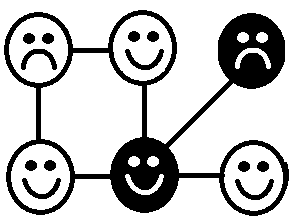
\includegraphics[width=0.6\linewidth]{happy-unhappy.png}
\caption{A cut that is not locally maximal.}
\end{figure}

%----------------------------------------------------------------------------------------

\end{column} 

%%%%%%%% END FIRST COLUMN %%%%%%%% 

\begin{column}{\sepwid}\end{column} % Empty spacer column

%%%%%%%% BEGIN SECOND COLUMN %%%%%%%% 

\begin{column}{\twocolwid}\vspace{-.8in} % Begin a column which is two columns wide (column 2)


\begin{block}{Quantum Approach}    
    
    We use the QAOA for the local \textsc{MaxCut} problem on $n$ vertices. Each run of the QAOA utilizes two tuples of angles $\gamma \in [0,2\pi]^p$ and $\beta \in [0, \pi]^p$ to construct gates resulting in a quantum circuit depth of $O(p)$. We construct diagonal Hamiltonian $C \in \mathbb{C}^{2^n \times 2^n}$ whose entries correspond to the number of happy vertices for each of the $2^n$ cuts. The standard mixing operator $B = \sum_{v} \sigma_x^{(v)}$ is used. We use the angles $\gamma = (\gamma_1, \dots, \gamma_p)$ and $\beta = (\beta_1, \dots, \beta_p)$ to construct state $\ket{\gamma,\beta} = e^{-i \beta_p B} e^{-i \gamma_p C} \cdots e^{-i \beta_1 B} e^{-i \gamma_1 C} \ket{+}_n$, where $\ket{+}_n = H^{\otimes n}\ket{0}$ is the uniform superposition. The problem reduces to finding $M(C):= \max\limits_{\gamma, \beta } \{ \braket{\gamma, \beta|C|\gamma,\beta} \}$.

    \begin{figure}[h]
          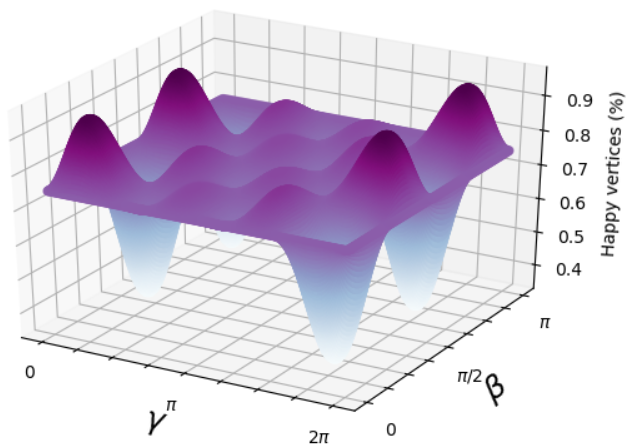
\includegraphics[width=0.8\textwidth]{statespace-1p-untitled.png}
          \caption{$M(C)$ for $p=1$ on $2$-regular graphs} 
          \label{fig:plot}
    \end{figure}
    
\end{block}

\vspace{-.8in}

\begin{block}{Classical Approach}
    We use a probabilistic algorithm with $p$ steps that acts on each vertex using only local information.

    \vspace{.3in}
    
	\begin{alertblock}{Theorem}
		There exists a classical local algorithm for local \textsc{MaxCut} such that after $p > 0$ steps on a $2$-regular graph, the expected fraction of happy vertices is at least $1 - (5/100)(1/2)^{p-1}$.
	\end{alertblock}


\end{block}


\end{column} % End of the second column



\begin{column}{\sepwid}\end{column} % Empty spacer column



\begin{column}{\onecolwid}\vspace{-.8in} % The third column

%----------------------------------------------------------------------------------------
%	RESULTS
%----------------------------------------------------------------------------------------

\begin{block}{Results}

    \begin{table}
        \begin{tabular}{|l | c | c | c | c |}
            \hline\hline \vspace{-.77in} \\
        $\boldsymbol{p}$ & 0 & 1 & 2 & 3 \\
        \hline \hline
        \textbf{Quantum} & 0.75 & 0.939 & 0.956 & \textcolor{blue}{0.956}\\
        \hline  \vspace{-.77in}\\
        \textbf{Classical} & 0.75 & 0.95 & 0.975 & 0.9875 \\ 
        \hline
        \end{tabular}
        \caption{The expected percentage of happy vertices on graphs with degree 2. The QAOA is non-decreasing as $p$ increases but our simulations have not found $\gamma,\beta$ resulting in improving expectation values for $p=3$.}
    \end{table}

\end{block}

%----------------------------------------------------------------------------------------
%	ADDITIONAL INFORMATION
%----------------------------------------------------------------------------------------

\vspace{-1.2in}
\begin{block}{Open Questions}


\begin{itemize}
\item How does the QAOA behave for large circuit depth on local \textsc{MaxCut}?
\item What is the relationship between approaches as graph degree increases?
\item Can we improve upon the the classical bounds with more in depth analysis or more complex algorithms?
\end{itemize}

\end{block}

%----------------------------------------------------------------------------------------
%	REFERENCES
%----------------------------------------------------------------------------------------

\vspace{-.8in}
\begin{block}{References}

% \nocite{*} % Insert publications even if they are not cited in the poster
\footnotesize{\bibliographystyle{abbrv}
\bibliography{bib}
% \vspace{0.75in}
}

\end{block}

% \vspace{-1in}
\begin{block}{Contact}

    \href{mailto:steven.kordonowy@colorado.edu}{steven.kordonowy@colorado.edu}
    
\end{block}




%----------------------------------------------------------------------------------------

\end{column} % End of the third column

\end{columns} % End of all the columns in the poster

\end{frame} % End of the enclosing frame

\end{document}
